\documentclass[14pt,a4paper,article]{ncc}
\usepackage[a4paper, mag=1000, left=2.5cm, right=1cm, top=2cm, bottom=2cm, headsep=0.7cm, footskip=1cm]{geometry}
\usepackage[utf8]{inputenc}
\usepackage[T2A]{fontenc}
\usepackage[russian]{babel} %[english,russian]
\usepackage{indentfirst}
\usepackage[dvipsnames]{xcolor}
\usepackage[pdftex,unicode=true,colorlinks,filecolor=black,citecolor=black,linkcolor=black]{hyperref}
\usepackage{amsfonts}
\usepackage{amsmath}
\usepackage{listings}
\usepackage{xcolor}

\usepackage{fancyhdr}
\pagestyle{fancy}
\fancyhead[LE,RO]{\thepage}
\fancyfoot{} 

\begin{document}
\begin{titlepage}
    \begin{center}
        САНКТ-ПЕТЕРБУРГСКИЙ ПОЛИТЕХНИЧЕСКИЙ УНИВЕРСИТЕТ ИМЕНИ ПЕТРА ВЕЛИКОГО \\
        \vspace{1em}
        \large Высшая школа прикладной математики и механики \\
        \large Кафедра прикладной математики и информатики \\ 
    \end{center}
    \vspace{8em}
    \begin{center}
        \textsc{\textbf{Лабораторная работа #1}}\\
    \end{center}
    \vspace{14em}
    \newbox{\lbox}
    \savebox{\lbox}{\hbox{Соломатин Макар Александр}}
    \newlength{\maxl}
    \setlength{\maxl}{\wd\lbox}
    \hfill\parbox{11cm}{
    \hspace*{5cm}\hspace*{-5cm}Студент:\hfill\hbox to\maxl{Макар Александрович Соломатин\hfill}\\
    \hspace*{5cm}\hspace*{-5cm}Преподаватель:\hfill\hbox to\maxl{Александр Николаевич Баженов}\\
    \\
    \hspace*{5cm}\hspace*{-5cm}Группа: \hfill\hbox to\maxl{3630102/70201}\\
    }
    \vspace{\fill}
    \begin{center}
        Санкт-Петербург \\2020
    \end{center}
\end{titlepage}

\tableofcontents
\newpage

\section{Постановка задачи}
Требуется найти $\varepsilon > 0$, при котором следующие интервальные
матрицы - особенные (содержат особенную точечную матрицу):
\begin{enumerate}
    \item 
    \begin{equation*}
    \textbf{A} = 
    \begin{pmatrix}
        [1 - \varepsilon, 1 + \varepsilon] & [1 - \varepsilon, 1 + \varepsilon] \\
        [1.1 - \varepsilon, 1.1 + \varepsilon] & [1 - \varepsilon, 1 + \varepsilon]
    \end{pmatrix}
    \end{equation*}
    
    \item 
    \begin{equation*}
    \textbf{A} = 
    \begin{pmatrix}
        1 & [0, \varepsilon] & \cdots & [0, \varepsilon] \\
        [0, \varepsilon] & 1 & \cdots & [0, \varepsilon] \\
        \cdots & \cdots & \cdots & \cdots \\
        [0, \varepsilon] & [0, \varepsilon] & \cdots & 1
    \end{pmatrix}
    \end{equation*}
\end{enumerate}

\section{Теория}
\textbf{Определение}. Интервальная матрицы -- прямоугольная таблиица, составленная из интервалов $\textbf{a}_{ij}: \textbf{A} = (\textbf{a})_{ij}$.


\textbf{Определение}. Вершинами интервальной матрицы $A = (a_{ij})$ из $\mathbb{IR}^{m\times n}$ назовем точечные $m \times n$-матрицы, $ij$-ым элементом которых
является $\underline{\textbf{a}}_{ij}$ или $\overline{\textbf{a}}_{ij}$. Множество вершин интервальной матрицы обозначим как 
$$ \text{vert} \textbf{A} := \{A \in \mathbb{R}^{m \times n}\;|\; A = (a_{ij}),\; a_{ij} \in \{\underline{\textbf{a}}_{ij}, \overline{\textbf{a}}_{ij}\}\} $$


\textbf{Определение}. Интервальная матрица $\textbf{A} \in \mathbb{IR}$ называется неособенной, если неособенны все точечные матрицы $A \in \textbf{A}$.
Интервальная матрица называется особенной, если она содержит особенную точечную матрицу.

\textbf{Теорема (критерий Баумана)}. Интервальная матрица \textbf{A} неособенна тогда и только тогда,
когда определители всех ее крайних матриц имеют одинаковых знак, т.е.
$$\forall A', A'' \in \text{vert} \textbf{A} \;\; (\text{det} A') \cdot (\text{det} A'') > 0$$


\textbf{Теорема (признак Бекка)}. Пусть интервальная матрица $\textbf{A} \in \mathbb{IR}^{m\times n}$ такова, что ее середина $\text{mid} \textbf{A}$ неособенна
и 
$$ \rho(|(\text{mid} \textbf{A})^{-1}| \cdot \text{rad} \textbf{A}) < 1 $$
Тогда \textbf{A} неособенна.


\section{Решение}
\subsection{Задача 1}
Для нахождения требуемого $\varepsilon$ воспользуемся критерием Баумана.
Найдем определители во всех вершинах этой интервальной матрицы.

$$\textbf{det A} = (1 \pm \varepsilon)^2 - (1.1 \pm \varepsilon)(1 \pm \varepsilon) = (1 \pm 1)\varepsilon^2 + (\pm 2 \pm 1.1 \pm 1)\varepsilon - 0.1$$

Наибольшего значения определитель достигает, когда 
\begin{equation}
\text{det} A = 2\varepsilon^2 + 4.1\varepsilon - 0.1    
\end{equation}

И наименьшего, когда
\begin{equation}
\text{det} A = -4.1\varepsilon - 0.1  
\end{equation}

По критерию Баумана, и.м. \textbf{A} будет неособенной, если
определители во всех вершинах имеют одинаковый знак, а значит
будет особенной, если есть определители с разными знаками.

Для этого необходимо и достаточно, чтобы наибольший определитель
(1)был больше нуля, а наименьший (2) был меньше нуля.

Решаем квадратное неравенство
\begin{equation}
 \begin{cases}
   2\varepsilon^2 + 4.1\varepsilon - 0.1 &> 0 \\
   -4.1\varepsilon - 0.1 &< 0
 \end{cases}
\end{equation}

Получаем
\begin{equation}
 \begin{cases}
   (\varepsilon + 2.074)(\varepsilon - 0.024) &> 0 \\
   \varepsilon &> 0.024
 \end{cases}
\end{equation}
С учетом $\varepsilon > 0$, матрица \textbf{A} является особенной
при $\varepsilon > 0.024$

\subsection{Задача 2}
Для решения задачи воспользуемся признаком Бекка. Будем искать минимальный $\varepsilon$, при котором 
в интервальную матрицу входит особенная матрица. Для этого возьмем отрезок $[0; 500]$ и будем
искать $\varepsilon$ методом половинного деления, проверяя середину очередного отрезка на условие
$$ \rho(|(\text{mid} \textbf{A})^{-1}| \cdot \text{rad} \textbf{A}) < 1 $$
Если середина отрезка такова, что матрица с ее радиусом -- неособенная, то сместим левую границу в середину отрезка,
иначе -- правую. Код программы приведен в Приложении.
Вычисленные значения $\varepsilon$ для некоторых $n$:

\begin{center}
\begin{tabular}{|c|c|}
\hline
n & $\varepsilon$ \\
\hline
2 & 1.000\\
3 & 0.594\\
4 & 0.419\\
5 & 0.323\\
6 & 0.262\\
7 & 0.213\\
8 & 0.182\\
\hline
\end{tabular}
\end{center}

График зависимости $\varepsilon(n)$:
\begin{figure}[h]
\center{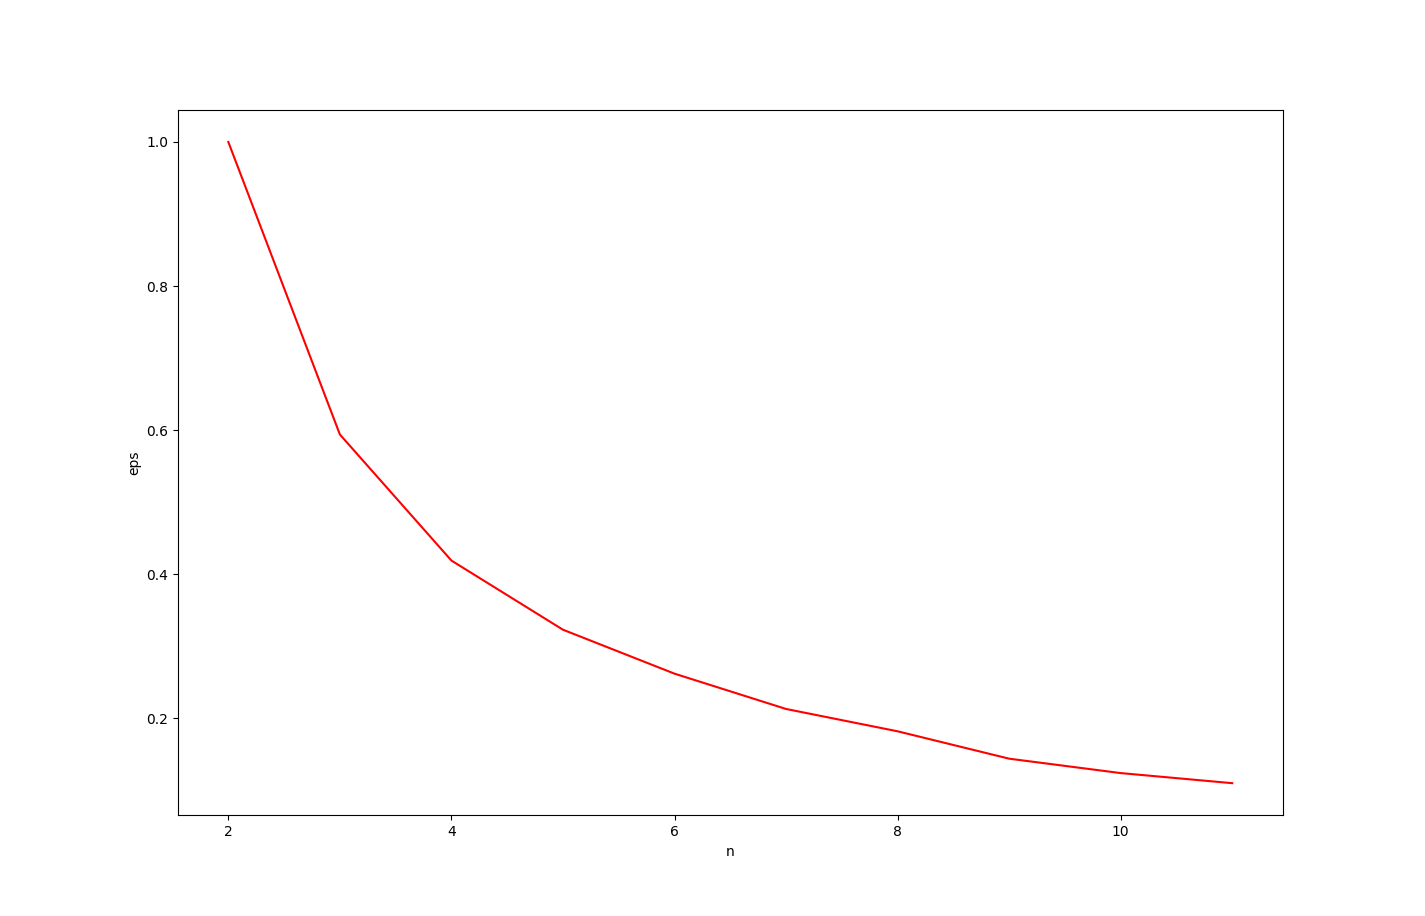
\includegraphics[scale=0.5]{Figure_1.png}}
\caption{Зависимость $\varepsilon(n)$}
\label{fig:image}
\end{figure}

\section{Вывод}
В первой задаче критерий Баумана легко применим - размерность интервальной матрицы всего лишь 2,
и можно составить выражение для определителя и его наибольшее и наименьшее значение в вершинах аналитически.
В задачах высокой размерности, количество вершин возрастает экспонентциально, и более рациональным будет 
использование признака Бекка.
Однако из-за приближенного вычисления обратной матрицы и спектрального радиуса, 
этот метод сам является приближенным.

Минимальная величина $\varepsilon$, при которой интервальная матрица во второй задаче начинает
быть особенной, как видно из графика, обратна пропорциональна размеру $n$ этой матрицы.
Можно объяснить это тем, что за счет увеличения количества интервальных элементов в матрице при
увеличении ее размера, множество различных определителей точечных матриц становится шире, а значит и охватывает $0$ при меньших магнитудах интервалов.

\section{Приложение}
\begin{enumerate}
    \item Репозиторий с исходным кодом \\ \url{https://github.com/MakarSolomatin/interval_analysis}
\end{enumerate}

\begin{thebibliography}{9}
    \bibitem{lectures} А. Н. Баженов. \textit{Лекции по интервальному анализу}.
\end{thebibliography}

\end{document}
